\section{Day 5: Induced Topologies (Sep. 17, 2024)}
Outfit of the day! Gives sushi shop california roll vibes :3
\begin{figure}[h]
    \centering
    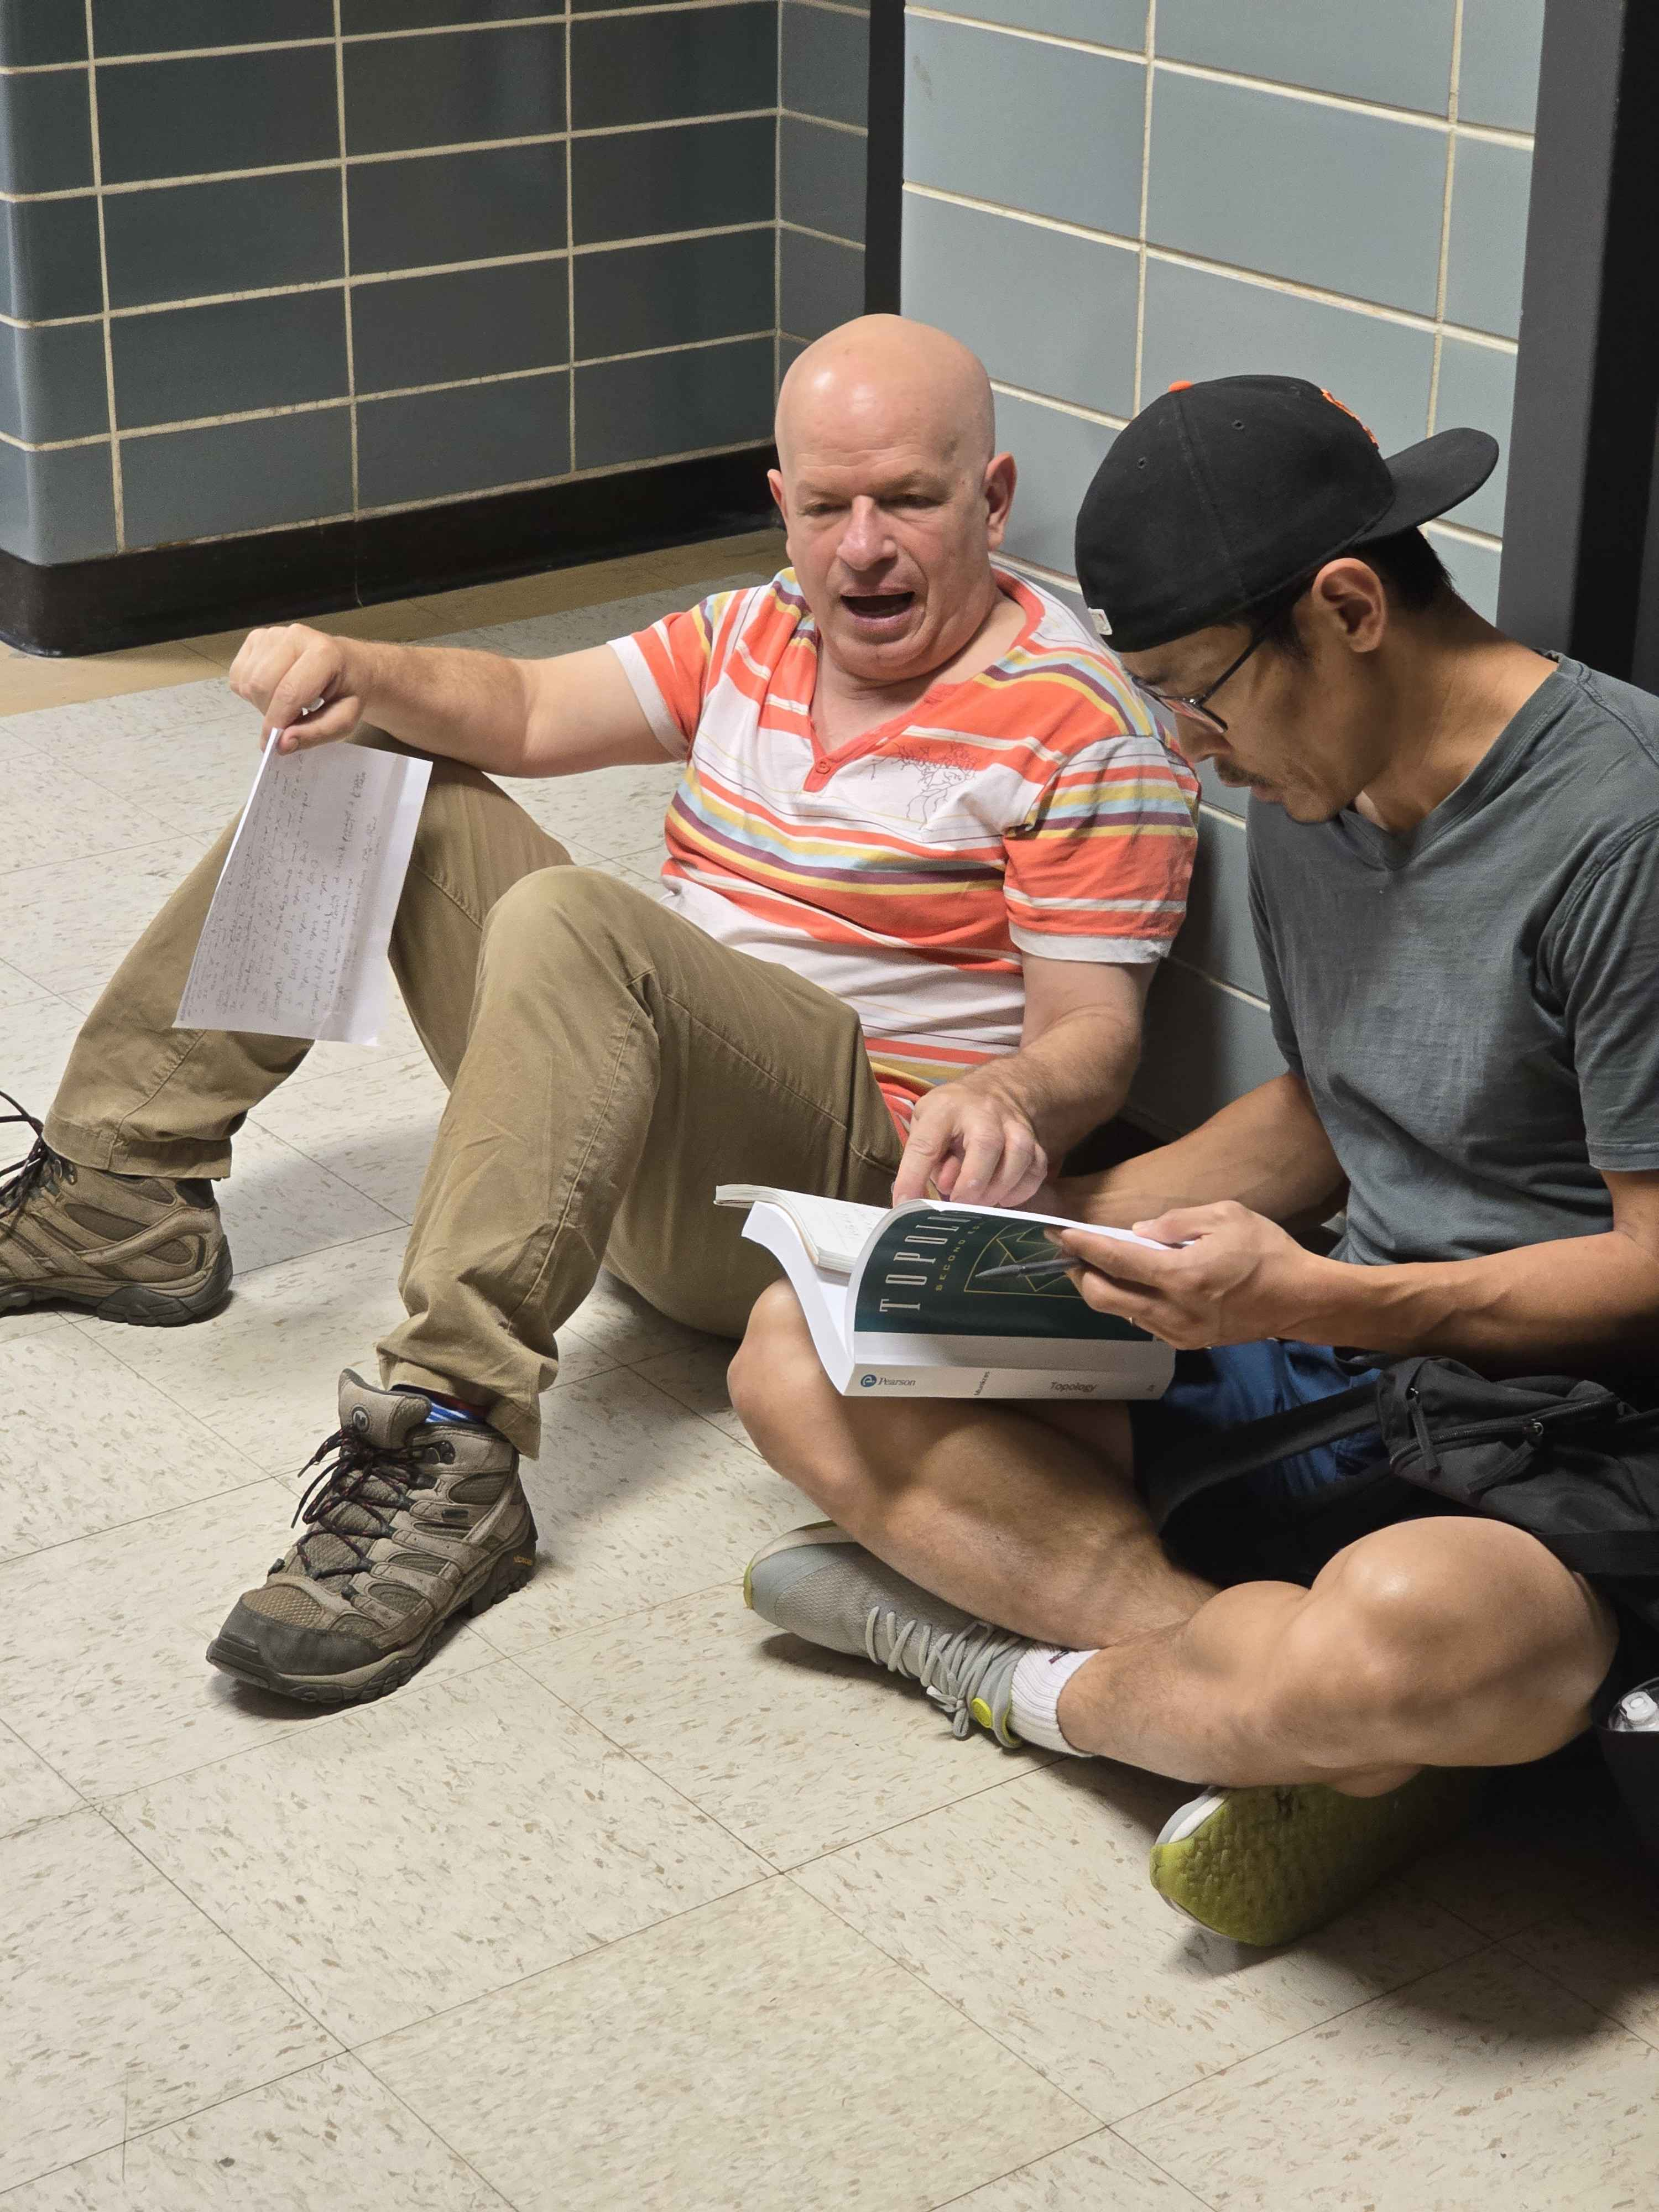
\includegraphics[scale=0.1]{MAT327 Notes/Dror Shirts/dror day 5 shirt.jpg}
\end{figure}

\noindent This week, we will cover sections 17 to 18 in Munkres, and the pre-reading for next week will be from section 19 to section 20. Now for recap;
\medskip\newline
\noindent Given topological spaces $(X, \ST_X)$ and $(Y, \ST_Y)$, we define the product topology $\ST_{X \times Y}$ on $X \times Y$ to be the unique topology with the properties
\begin{enumerate}
    \item The projections $\pi_X : X \times Y \to X$ and $\pi_Y : X \times Y \to Y$ are continuous.
    \item For any function $h : Z \to X \times Y$, if $\pi_X \circ h, \pi_Y \circ h$ are continuous, then so is $h$.
\end{enumerate}
Moreover, we have that $\SB = \{U \times V \mid U \in \ST_X, V \in \ST_Y\}$ is a basis for $\ST_{X \times Y}$.
\begin{remark}[Homeomorphism to Cartesian Product with Singleton]
    Any topological space $X$ is homeomorphic to $X \times \{\ast\}$, where $\{\ast\}$ is some singleton. It is also homeomorphic to $\{\ast\} \times X$.
\end{remark}

\newpage
\noindent We now introduce the subspace topology (ref: section 16, Munkres). Given $(X, \ST_X)$ and some subset $Y \subset X$, we wish to construct a topology on $Y$ such that
\begin{enumerate}
    \item The inclusion map $\iota_Y : Y \xhookrightarrow{} X$ is continuous.\footnote{dror uses $i_Y$ instead of iota}
    \item If $f : Z \to Y$ has that $\iota_Y \circ f$ is continuous, then $f$ is also continuous.
\end{enumerate}
\begin{simplethm}[Subspace Topology Exists and is Unique]
    The topology on $Y$ satisfying the above two properties exists and is unique.
\end{simplethm}
\noindent We start with existence; let us claim that $\ST_Y := \{ \iota_Y^{-1}(U) = Y \cap U \mid U \in \ST_X \}$ satisfies the above two properties.
\begin{enumerate}
    \item By construction of the set, $\iota_Y$ is obviously continuous.
    \item If $f : Z \to Y$ and $\iota_Y \circ f$ is continuous, then let us take any open $V \in Y$, and consider $f^{-1}(Y)$. Pick $U \in \ST_X$ such that $V = U \cap X$. Then we have
    \[ f^{-1}(V) = f^{-1}(U \cap X) = f^{-1}(\iota_Y^{-1}(U)) = (\iota_Y \circ f)^{-1} (U). \]
    Since $\iota_Y \circ f$ is continuous, we have that $(\iota_Y \circ f)^{-1} (U)$ is open, and so we conclude $f$ is continuous. This concludes that $\ST_Y$ satisfies the properties.
\end{enumerate}
To prove uniqueness, suppose we have $\ST_Y'$ and $\ST_Y''$ satisfying the above two properties. Then observe the commutative triangle,
\[ \begin{tikzcd} && X \\ \\ {(Y, \ST_Y')} &&&& {(Y, \ST_Y'')} \arrow["{\iota_Y'}", hook, from=3-1, to=1-3] \arrow["Id"', tail reversed, from=3-1, to=3-5] \arrow["{\iota_Y''}"', hook', from=3-5, to=1-3] \end{tikzcd} \]
We have that $\iota_Y'' \circ \mathrm{Id} = \iota_Y'$; by proposition $1$ of $\ST_Y'$, we have that $\iota_Y'$ is continuous, meaning $\iota_Y'' \circ \mathrm{Id}$ is as well. By proposition $2$ of $\ST_Y''$, this means the identity between $(Y, \ST_Y')$ and $(Y, \ST_Y'')$ is continuous, concluding that $\ST_Y' = \ST_Y''$. \qed
\medskip\newline
\noindent We now give some examples of subset topologies.
\begin{enumerate}[label=(\alph*)]
    \item Consider $[0, 1] \subset \RR$ (where we identify $Y$ with $[0, 1]$ and $\RR$ with $X$).\footnote{Note that the convention is that if the topology on $\RR$ is not specified, then it is automatically the standard topology $\RR_\mathrm{std}$.} Then the topology $\ST_{[0, 1], \mathrm{std}}$ is given by $\{ U \cap [0, 1] \mid U \in \RR_\mathrm{std} \}$. Note that we may consider a subset topology on $\RR$ even if $Y$ is not a open set.
    \medskip\newline
    If $Y \subset X$ is an open set, then open sets in $\ST_Y$ are automatically open in $X$ as well.
    \item Now, suppose $Y' \subset Y$ and $X' \subset X$. Then $X' \times Y'$ has two topologies:
    \begin{enumerate}[label=(\alph*)]
        \item As a subset of the product topology $X \times Y$,
        \item As a product of two subsets, one of $X$ and the other of $Y$.
    \end{enumerate}
    We claim that these topologies are the same. \textit{(Originally left as exercise.)}
    \item Let us have $Z \subset Y \subset X$. Let $Y$ have the subspace topology induced by $X$, and let $Z$ have the subspace topology induced by $Y$. Then $Z$ also has subspace topology induced by $X$.
\end{enumerate}

\newpage
\noindent We now give some examples of product topologies.
\begin{enumerate}[label=(\alph*)]
    \item Let us have the product topologies $X \times Y, Y \times X$. Is $X \times Y = Y \times X$? Not necessariy, but we may construct a homeomorphism between them (by swapping coordinates). Note that this is different; if we induce an order topology on $X \times Y$ and $Y \times X$, then this is almost never true.
    \item Let $X, Y, Z$ be topological spaces. Then the cartesian product $(X \times Y) \times Z \neq X \times (Y \times Z)$
    is generally not associative, since the sets have structure $\{((x, y), z)\}$ and $\{(x, (y, z))\}$. However, it is common to identify both of them as $X \times Y \times Z$ as an abuse of notation, with elements $\{(x, y, z)\}$. Thus, the product of finitely many topological spaces makes sense from induction on above, i.e.
    \[ X_1 \times \dots \times X_n. \]
\end{enumerate}

\noindent In general, induced topologies interact well with bases; for example, $\ST_{X \times Y}$ is the topology generated by $\{U \times V \mid U \in \ST_X, V \in \ST_Y\}$. In terms of basis, we may write $\SB = \{U \times V \mid U \in \SB_X, V \in \SB_Y\}$ with bases $\SB_X, \SB_Y$ from $X, Y$ respectively.
\medskip\newline
The subspace topology $Y \subset X$ also interacts well with bases, i.e. $\SB_Y = \{Y \cap B \mid B \in \SB_X\}$. One of the only situations that the subspace topology does not work well with bases is with the order topology; let $X$ be ordered, and let $Y \subset X$. Then $Y$ can either inherits order or topology from $X$. Suppose these two are called by $Y_\mathrm{ord}$ and $Y_\mathrm{subs}$. Sometimes, $Y_\mathrm{ord} \neq Y_\mathrm{subs}$, but they are equal if $Y$ is convex. This example is gone over in Munkres.\footnote{yeah i'm confused here.}